\chapter{Progetto e attività di stage}
\textit{Questa capitolo parla delle attività di stage andando a descrivere il progetto nei suoi stati di avanzamento, le scelte adottate e le motivazioni che mi hanno permesso di scegliere.}

\section{Formazione}
All'inizio dello stage, la prima attività che ho dovuto svolgere è stata quella di studio delle applicazioni adottate dall'azienda e i formalismi, ovvero codici e abbreviazioni adottate per la realizzazione dei campi di database. 
Per la formazione sull'applicazione \inde\, ho seguito sei video-corsi della durata di una o anche due ore l'uno. In aggiunta, per velocizzare l'apprendimento dell'uso dell'applicazione, è stato richiesto che venissero realizzate le applicazioni presenti nei video.
Rispetto a quanto pianificato, l'apprendimento del programma è risultato più rapido della settimana preventivata e quindi, durante la stessa, ho potuto interfacciarmi con i data warehouse e lo studio di alcune stored procedure. 
Verso fine settimana ho iniziato lo studio dei documenti relativi al configuratore catalogo/prodotti.


\section{Progettazione}
Dalla seconda settimana di stage, ho iniziato ad affrontare le dinamiche aziendali concentrandomi nelle attività di progetto che è stata divisa in incontri con il cliente e lavoro presso la sede di Castelfranco.

\subsection{Database}
Affiancato al tutor aziendale, il primo punto affrontato è stato il database. Il cliente ci ha dato carta bianca, ovvero potevamo decidere tra due soluzioni: riutilizzare tabelle presenti nel database oppure crearne di nuove. Questo cliente specifico dispone tra i suoi software di sei applicazioni ideate con InDe e nei mesi di stage hanno iniziato a chiedere nuovi progetti.

La scelta, dopo una attenta discussione con il cliente, è stata quella di creare delle tabelle nuove perché questa nuova componente in futuro vorrebbero integrarla in altre applicazioni oltre che a quella per cui è stata realizzata.\\
Per cercare di mantenere una certa uniformità con il resto del data warehouse, la prima scelta è stata quella di non inserire vincoli di Foreign Key.
Questo vincolo che avrebbe permesso query più rapide è risultato superfluo in seguito alla velocità dei server. Tuttavia, continuo a ritenere molto utile la creazione delle foreign key perché in questo modo se anche le tabelle iniziano ad avere una quantità di record spropositata la velocità resta soddisfacente. Inoltre, il problema dell'eventuale plugin dell'applicazione richiede comunque che si metta mano al codice nell'importazione della componente. 
Quest'ultima scelta ha portato il vantaggio di estendere i progetti in maniera più rapida.
Infine, per concludere il tema vincoli gli unici adottati sono quelli di Primary Key.
\\

La prima tabella da cui partire è quella dedicata agli articoli. Quest'ultima è già presente nel data warehouse e dispone di una vista. Partendo da questi due contenitori, si è realizzata una struttura che permetta prima di realizzare una lista prodotti, poi, se l'articolo esiste, arricchire le sue informazioni.\\

Gli aspetti da tenere in considerazione sono stati:
\begin{itemize}
	\item ogni articolo ha delle immagini, video o dei file di vario genere;
	\item ogni articolo deve poter avere uno o più tag;
	\item ogni articolo deve avere delle informazioni di base e delle informazioni aggiuntive;
	\item ogni informazione aggiuntiva deve poter essere gestita (creata, modificata ed eliminata).
\end{itemize}
Queste informazioni sono state definite durante la prima riunione presso la sede del cliente.\\

\begin{figure}[!h] 
	\centering 
	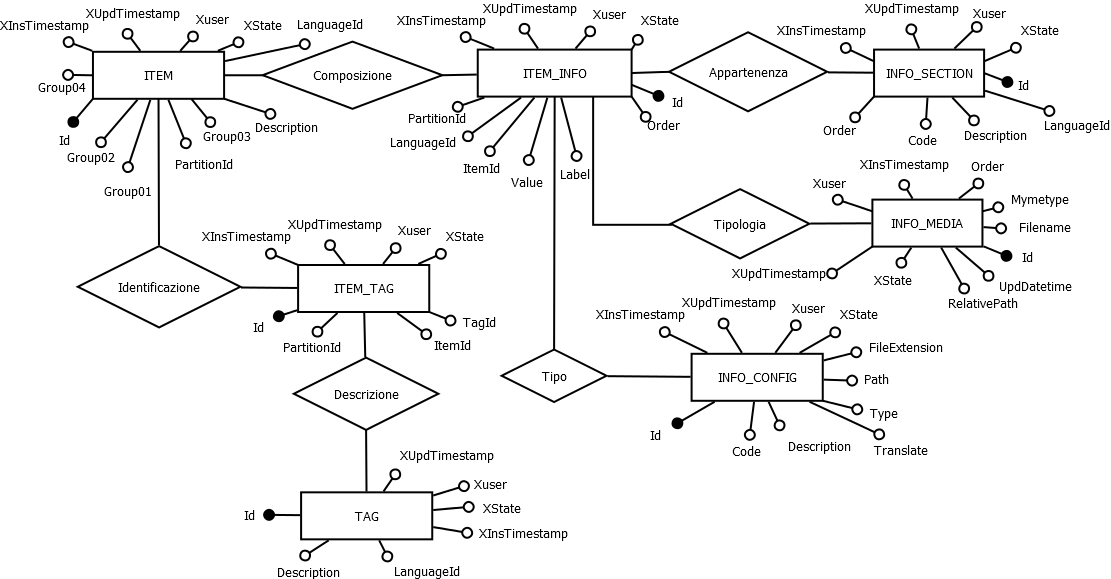
\includegraphics[width=1\columnwidth]{DiagrammaER} 
	\caption{Diagramma Entity Relationship}
	\label{DiagrammaER}
\end{figure}

Il diagramma ER (i vincoli sono fittizi, mostrano i collegamenti nonostante l'assenza di foreign key) è stato pensato in modo tale che ogni articolo dispone di molte informazioni e ciascuna di esse appartiene ad una categoria.

\paragraph{ITEM}
Questo oggetto è una vista con alcune delle informazioni più importanti. Visto che la fase di inserimento prevede unicamente che un'utente possa inserire alcune informazioni. I dati gestiti nella vista sono i gruppi di appartenenza (ad esempio insaccati, surgelati, prodotti da forno) ed una descrizione breve dell'oggetto.
In questo contesto la descrizione appare due volte una negli ITEM ed una nella ITEM\_INFO per il semplice motivo che la tabella esisteva già nel database.

\paragraph{ITEM\_INFO}
Nella seguente tabella vengono raccolte tutte le informazioni e rappresenta il punto di collegamento dell'intero progetto. In esso vengono inserite le etichette e i valori che rappresentano i punti fondamentali di questa tabella. Le etichette (label) sono la descrizione dei valori (value) che permettono ricerche in tabella più rapide (video, titolo, immagine). I valori sono quelli che in base alle altre tabelle saranno stampati a video dall'applicazione web di front-end (\hyperref[frontend]{figura \ref{frontend}}).

\paragraph{INFO\_CONFIG}
La tabella INFO\_CONFIG è stata realizzata al fine di inserire record con specifiche che limitano i tipi di record che possono essere gestiti all'interno di ITEM\_INFO. Inoltre definiscono le caratteristiche su cui sono fondati i record della tabella associata ad esempio è possibile definire le estensioni di file o un parametro che mi hanno chiesto di gestire in un secondo momento, ovvero la lingua; nel diagramma risulta già presente, ma in realtà è stato aggiunto in un secondo momento verso fine progetto circa a metà della penultima settimana.

\paragraph{INFO\_MEDIA}
INFO\_MEDIA è la tabella, come è comprensibile dal nome, che detiene tutte le informazioni relative ai file. In questo caso una prima idea è stata quella di salvare il file nel database con un blob, tuttavia ho pensato che poi nell'interrogazione di una tabella contenente molti media poteva diventare molto pesante considerando la richiesta di gestione dei video. In questa occasione ho pensato fosse più propizio ideare una cartella online dove è installata l'applicazione con un GUID (nome univoco) assegnato al file e nel database disporre unicamente del percorso relativo dell'immagine.

\paragraph{INFO\_SECTION}
Le informazioni relative ad un prodotto devono essere categorizzate. Questa tabella ha la funzione di indicare la categoria di appartenenza così come avviene in diversi siti e-commerce. L'idea è di poter gestire le informazioni presentandole in sezioni dinamiche tante quante si ritengano necessarie. 

\paragraph{TAG}
Tabella che serve ad includere ogni tipo di parole chiavi che permettano di effettuare ricerche per arrivare ad uno specifico prodotto o gruppo di prodotti. Questa tabella non è stata creata perché è adoperata in altri contesti.

\paragraph{ITEM\_TAG}
Quest'ultima tabella ha lo scopo di collegare i tag con lo specifico articolo. Si è di fronte ad una relazione uno a molti che, in fase di ristrutturazione, ha comportato la creazione di una tabella intermedia tra articoli e tag.



\subsection{Design Pattern}
Nella realizzazione dell'applicazione per la maggior parte delle videate un singolo oggetto doveva gestire le sue operazioni nella propria videata. Vi è stato solo un caso particolare che ha richiesto l'uso di un design pattern e che già nella fase di progettazione del database è stato abbozzato: nella gestione di dettaglio del singolo articolo.
Il pattern scelto è il Facade. Tutte le informazioni partono da un articolo (record della tabella ITEM) e da questo vengono generate opportune operazioni.\\

\begin{figure}[!h] 
	\centering 
	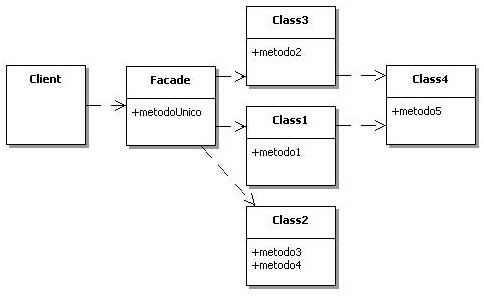
\includegraphics[width=1\columnwidth]{Pattern} 
	\caption{Design pattern strutturale: Facade (\url{https://bit.ly/2McTHsR})}
	\label{Pattern}
\end{figure}


Il grafico UML generato una volta definito il design pattern da applicare è risultato essere quello sottostante. Per realizzarlo, ho seguito la logica che doveva avere l'applicazione ed ho provato a segnare le attività di caricamento, creazione, modifica e cancellazione dei record delle diverse tabelle.

\begin{figure}[!h] 
	\centering 
	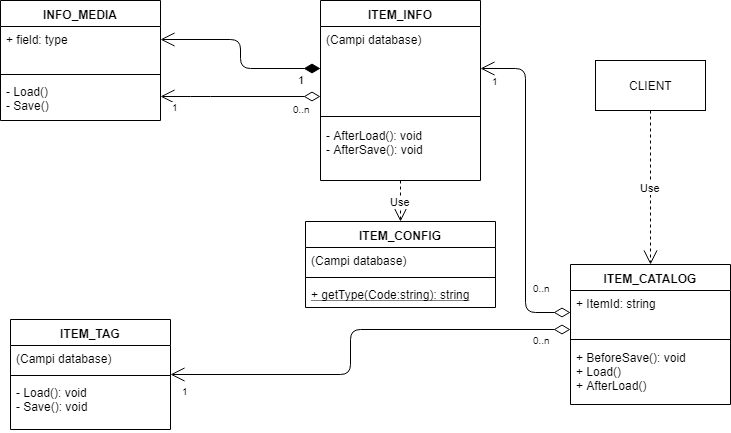
\includegraphics[width=0.7\columnwidth]{UML2} 
	\caption{Diagramma UML delle classi}
	\label{UML}
\end{figure}

%\subsubsection{Diagrammi di sequenza}
\paragraph{Caricamento}
Un dettaglio articolo non è altro che un'insieme di informazioni (ITEM\_INFO). Partendo da questo presupposto ho deciso di caricare un array di oggetti (in InDe prende il nome di IDCollection).
Per definire quale articolo caricare indico uso l'id dell'articolo; quindi carico le varie informazioni tramite query. Quando ricevo una informazione verifico immediatamente a quale configurazione (INFO\_CONFIG) appartiene e solo se necessario carico gli ulteriori dati, ovvero i media. Infine, con la classe ITEM\_TAG metto in un array tutti i tag associati all'articolo selezionato.

\paragraph{Creazione}
Questa operazione è molto più semplice e controllata. Prima creo un articolo (ITEM), quindi entro nel dettaglio e creo tanti ITEM\_INFO con o senza il proprio ITEM\_MEDIA. Poi se vengono inseriti creo gli ITEM\_TAG. Tutto questo viene salvato unicamente dall'oggetto ITEM\_CATALOG che fa partire gli eventi di save dei vari oggetti.

\paragraph{Modifica}
In questo caso la modifica è uguale all'inserimento. La differenza è che in inserimento all'inizio devo creare un articolo e poi aprire il suo dettaglio senza caricare informazioni. In questa situazione, l'oggetto deve caricare ogni singola informazione quindi è necessario un controllo sulle query se ritornano o meno informazioni. In seguito, cambiando un dato questo segnala all'oggetto, a volte forzando l'update, che devono essere aggiornati i dati.

\paragraph{Cancellazione}
L'ultima operazione non meno importante è la cancellazione. Questa deve generare la cancellazione di ogni singolo record di uno specifico articolo senza lasciare record "orfani". Per evitare questo fenomeno, quando cancello inizio dai figli fino al raggiungimento del padre ed infine blocco la cancellazione dell'articolo (ITEM), ma cambio lo stato di un campo del record da "I" (Insert) o "M"(Modified) a "D" (Deleted) ed aggiorno XUpdDatetime.


\todo diagrammi di sequenza per le 4 operazioni


\section{Codifica}
Dopo la fase di progettazione, si è affrontata la codifica. Questa fase è stata differente rispetto a quanto ho sviluppato durante il corso di Programmazione ad oggetti, Programmazione concorrente e distribuita ed Ingegneria del Software. Il motivo della diversità è l'applicazione \inde.\\
Progettare classi e videate con questo software mi ha abbastanza cambiato il modo di implementare e testare. Prima di questo cambiamento tendevo a crearmi una scaletta, implementarla e passo per passo effettuare dei test di unità basati su codice scritto (ad esempio Java associato a JUnit).\\
In questo contesto, invece, mi sono ritrovato a saltare i test di unità e passare immediatamente a test di sistema. Di conseguenza ho creato classi, metodi ed eventi cercando quanto più possibile di seguire una logica rigorosamente commentata. Mi attendevo molti errori, ma sono rimasto sorpreso. Il numero di errori, per il fatto che il codice generato si basa su template ben controllato e già testato dalla casa produttrice, era molto basso e, con il debugger incluso, ho potuto risolvere ogni errore commesso in poco tempo per poi passare ad altre funzionalità.

\subsection{Documenti}
\inde\ definisce con il termine documenti le classi java o c\# che dovranno essere generate e da cui si basano le applicazioni ideate.
Le prime classi che ho creato sono state quelle automatiche, secondo il ragionamento del framework ORM di InDe. Ho preso le tabelle del database e implementato una classe per ciascuna. Il funzionamento di alcune delle classi è rimasto quello standard. La classe che ha richiesto un ragionamento maggiore è stata quella per la gestione del dettaglio articoli.
La creazione automatica genera delle classi con tanti attributi quanti sono quelli presenti nelle tabelle di riferimento e con essi sono creati anche i metodi get e set, rispettivamente dedicati a mostrare e modificare i valori di un record.

A seguito dell'utilizzo dell'ORM, le classi vengono generate sulla base di un template. Tutte le classi basate su un database estendono una classe IDDocument la quale contiene ogni metodo necessario ed evento necessario da gestire. Nelle classi derivate, create a partire da una tabella, è possibile intravedere nel codice come solo i metodi ed eventi di cui si hanno la necessità sono valorizzati e ridefiniti, mentre gli altri metodi previsti dal programma sono solo dichiarati e riprendono il funzionamento della classe padre.

\subsubsection{ITEM}
La classe dedicata all'articolo è rimasta pressoché invariata. \'E stato creato un campo decodifica gruppi al fine di mostrarlo a video e popolarlo solo in caso di esigenza e si è rivista la query da cui vengono estrapolati i dati da assegnare ad un oggetto.

\begin{center}
	\begin{tabular}{ p{3cm}|p{9,2cm} }
		\hline
		\textbf{Metodo e Query} & \textbf{Descrizione}\\
		\hline
		BeforeSave() & Questo metodo rientra tra quelli generati automaticamente dal programma. Al suo normale funzionamento ho aggiunto alcune informazioni da salvare in caso di inserimento, modifica o cancellazione (XState, XInsTimestamp, XUpdTimestamp). Nella cancellazione ho bloccato l'operazione di "delete" trasformandola in una "update" in cui il valore XState passa a "D".\\
		\hline
		DecodificaGruppi() & Il metodo di decodifica gruppi è stato realizzato al fine di caricare in un campo di tipo string l'insieme dei gruppi di appartenenza dell'Articolo decodificando il codice nella descrizione corrispondente.\\
		\hline
		Master Query & Le master query sono le query di base che vengono lanciate per popolare gli attributi di una classe. In questo caso la modifica è stata quella di limitare la visibilità ai soli record il cui campo XState non fosse "D", ovvero cancellato.\\
	
	\end{tabular}

\end{center}

\subsubsection{ITEM\_INFO}
Per quanto riguarda le informazioni, mi sono dedicato molto al comportamento che l'oggetto dovrebbe avere durante l'esecuzione dell'applicazione web. Dopo la lettura e salvataggio dei dati nel database. 
\begin{center}
	\begin{tabular}{ p{3cm}|p{9,2cm} }
	%	\hline
	%	\multicolumn{2}{|c|}{ITEM\_INFO} \\
		\hline
		\textbf{Metodo e Query} & \textbf{Descrizione}\\
		\hline
		AfterSave() & Dopo aver salvato un oggetto di tipo ITEM\_INFO nel database, viene azionato questo metodo che ho utilizzato per controllare se l'informazione salvata è un'immagine e in quel caso procedere all'inserimento di alcuni valori nell'oggetto Media e salvarlo.\\
		\hline
		AfterLoad() & Come per la AfterSave(), dopo aver caricato la mia informazione verifico di che tipo è e se si tratta di una immagine la carico nell'oggetto Media interno alla classe.\\
		
	\end{tabular}
\end{center}

\subsubsection{ITEM\_CONFIG}
La ITEM\_CONFIG è stata tra le prime classi ad essere realizzata. Sulla base di questa sono gestiti alcuni eventi dell'ITEM\_INFO e dell'ITEM\_CATALOG. \'E stata studiata per contenere le configurazioni e ottenere in maniera rapida delle informazioni da altri oggetti. Per fare ciò ho creato metodi statici che effettuano query e ritornano una specifica informazione.
\begin{center}
	\begin{tabular}{ p{3cm}|p{9,2cm} }
		%	\hline
		%	\multicolumn{2}{|c|}{ITEM\_INFO} \\
		\hline
		\textbf{Metodo e Query} & \textbf{Descrizione}\\
		\hline
		BeforeSave()		& Come per l'articolo anche in questo caso la cancellazione è stata gestita a livello logico.\\
		\hline
		GetFileExtension(string code)	& Metodo statico che restituisce un valore booleano in base al tipo di estensione se accettata o meno.\\
		\hline
		GetPath(string code) & Metodo statico che restituisce il percorso dove salvare i tipo (code) di file.\\
		\hline
		HasModal(string code) & Metodo che mi permette di controllare se questo tipo di ITEM\_CONFIG deve essere o meno gestito con l'uso delle modali.\\

	\end{tabular}
\end{center}

\subsubsection{INFO\_MEDIA}
La classe dedicata alla gestione dei media ha richiesto molto tempo più che al caricamento dei file al suo salvataggio. In fase di inserimento record nel database ho anche dovuto trovare un modo per salvare le immagini in una cartella dell'applicazione web con un nome univoco.
\begin{center}
	\begin{tabular}{ p{4,2cm}|p{8cm} }
		\hline
		\textbf{Metodo e Query} & \textbf{Descrizione}\\
		\hline
		OnEndTransaction() & Metodo che viene richiamato ogni qual volta si crea o modifica un singolo campo del database che generalmente serve a popolare alcuni campi obbligatori ma non visibili. In questo caso è utilizzata per generare in automatico un path assoluto per permettere il caricamento dell'immagine. \\
		\hline
		BeforeSave()	& Prima di salvare il record controllo se esiste già il file nella directory di destinazione e verifico che non sia uguale all'immagine che ho caricato in modo da ridurre il i byte da trasferire ai soli necessari.\\
		\hline
		AfterLoad()	& Carico il percorso assoluto dell'immagine e verifico se è presente una immagine in quel percorso. La assegno ad una variabile che a video verrà immediatamente esposta.\\
		\hline
		GetMediaPath()& Metodo per ottenere il path dell'immagine.\\
		\hline
		ValorizzaImagePath(string TempPath)	& Metodo dedicato per creare una immagine temporanea nella cartella temporanea del programma che appena viene chiuso vengono cancellati automaticamente.\\
	
	\end{tabular}
\end{center}

\subsubsection{INFO\_SECTION e TAG}
Le seguenti due classe hanno mantenuto la gestione automatica generata da InDe. Tuttavia, anticipando quanto richiesto in un secondo momento, esposto nella sezione \ref{altriInterveti}, la classe INFO\_SECTION ha subito un cambiamento. Il cambiamento in questione è relativo alla gestione della lingua, che come in altre classi, ha introdotto dei nuovi controlli.

\subsubsection{ITEM\_TAG}
La classe è rimasta pressoché invariata da quella auto-generata nella gestione degli eventi fatta eccezione per l'inserimento e la modifica che ha richiesto solo l'arricchimento di dati di controllo.

\begin{center}
	\begin{tabular}{ p{3cm}|p{9,2cm} }
		%	\hline
		%	\multicolumn{2}{|c|}{ITEM\_INFO} \\
		\hline
		\textbf{Metodo e Query} & \textbf{Descrizione}\\
		\hline
		BeforeSave& Gestisco i campi XInsTimestamp, XUpdTimestamp e XState.\\
		\hline
		ExistsInCollection(IDCollection coll) & Metodo pubblico che controlla se un elemento è presente nella IDCollection.\\
		
	\end{tabular}
\end{center}

\subsubsection{ITEM\_CATALOG}
Questa classe funge da tramite per tutte le operazioni realtive al dettaglio di un prodotto. Essa non è basata su alcuna tabella. Nel caricamento delle informazioni vi sono specifiche query ideate per caricare unicamente la combinazione dei dati di un articolo. Si compone di due IDCollection una di ITEM\_INFO e una di ITEM\_TAG. La prima la utilizza per salvare le informazioni che vengono passate, mentre la seconda salva i tag.

\begin{center}
	\begin{tabular}{ p{3cm}|p{9,2cm} }
		%	\hline
		%	\multicolumn{2}{|c|}{ITEM\_INFO} \\
		\hline
		\textbf{Metodo e Query} & \textbf{Descrizione}\\
		\hline
		BeforeSave()& Questo evento ha in sè tutto il codice relativo all'inserimento, modifica e cancellazione dei dettagli articolo. Esso prende le informazioni passate dalle interfacce e richiama il salvataggio dei singoli ITEM\_INFO ed ITEM\_TAG indicando eventuali logiche a supporto.\\
		BeforeLoad()& L'oggetto non si basa su una tabella o query. Esso fa riferimento a due collezioni di oggetti. Per caricare le due collezioni ho inserito dei campi obbligatori: ItemId, per riconoscere l'articolo, combinato al partitionId, anche se ad oggi non è mai stato valorizzato.  \\
		
	\end{tabular}
\end{center}


\subsection{Videate}
La creazione delle interfacce utente, o come le chiamano su Instant Developer "Videate", ha richiesto un lavoro di "drug and drop". Quindi l'aspetto grafico è stato molto semplice e rapido, fatta eccezione per l'aspetto responsive che ha richiesto una combinazione tra le funzionalità di InDe e l'importazione di un foglio di stile (Cascading Style Sheet) customizzato.
I metodi gestiti nelle videate sono gli eventi di load, refresh, update (che comprende inserimento, modifica e cancellazione dei record).\\

Di tutte le videate realizzate, quelle più complesse sono state le interfacce dedicate al caricamento delle immagini. Nella loro realizzazione hanno richiesto la gestione di alcuni comportamenti a livello di applicazione generale differenti dall'usuale.
Il media ha richiesto delle continue rivisitazioni. Per la gestione dei file, il programma prevede che questi vengano caricati in una cartella temporanea. Tuttavia, da quanto si è definito in progettazione, una immagine viene salvata in una cartella ad essa dedicata con un nome univoco ideato solo per quello specifico elemento. 
Prima di arrivare ad una soluzione ho dovuto creare dei progetti di test e verificare pregi e difetti. La soluzione che ho individuato è stata combinare dei metodi dell'applicazione. Ho combinato il tempPath, metodo che restituisce il una stringa con il percorso alla cartella temporanea e il replace, metodo per il rimpiazzo di stringhe. Infine, con un makeDirectory, altro metodo di InDe ho creato il nuovo percorso dove salvare i file in maniera dinamica. 
L'insieme di questi metodi sono serviti a creare un nuovo percorso di salvataggio dei file, per caricarli effettivamente ho optato per una doppia gestione: trascinamento dell'immagine nell'applicazione oppure click nella sezione di drop-down e importazione standard di documenti dal computer alla pagina web. Infine, per il caricamento ho optato per caricarli nella cache in modo tale da caricare i media di un elemento una sola volta per l'intera durata della sessione.\\

L'ultimo aspetto di focale importanza è risultato essere il controllo dell'evento onCommand(), ovvero l'evento lanciato ogni qual volta si prema un pulsante presente nella intestazione della videata (refresh, save, insert, duplicate) assieme al comando load(), dedicato al caricamento delle videate ed a eventuali controlli prima di aprire una qualsiasi schermata.
La gestione degli onCommand(), rispetto a quanto aspiravo di creare, è stata diversa per ogni videata tuttavia il comportamento generale dell'applicazione ho cercato di standardizzarlo seguendo i seguenti principi:
\begin{itemize}
	\item da una lista posso inserire, modificare e cancellare solo le principali informazioni;
	\item da una lista posso entrare nel dettaglio di un singolo elemento;
	\item dal dettaglio posso inserire dati, modificarli e cancellarli;
	\item dal dettaglio posso caricare media o dati particolari solo attraverso modali controllate (ade esempio nelle mail viene controllato che ci siano parole separate dal simbolo di \@ e da un punto).
\end{itemize}


\subsubsection{Modali}
Le modali sono videate di dimensioni ridotte, paragonabili ai popup, nelle quali ho dovuto gestire il caricamento di diverse informazioni. Per evitare di adottare una classe non basata su una tabella per ciascuna delle videate ho adottato le tabele IMDB. 
Una tabella IMDB è una sorta di contenitore temporaneo che mantiene le sue informazioni fino al termine della sessione. Queste tabelle possono avere uno o più record così come possono essere utilizzate per effettuare dei filtri quando si apre una videata. Un esempio di suo utilizzo è stato l'inserimento delle variabili ItemId e PartitionId per filtrare un particolare articolo ed entrare quindi nel dettaglio di un singolo elemento.
Queste schermate sono state ideate al fine di passare dati alle videate sottostanti e si cancellano, alla chiusura, per non occupare memoria nella cache.


\section{Verifica, validazione e collaudo}
Le operazioni di verifica , validazione e collaudo sono risultate più semplici di quanto mi aspettassi. Per verificare il prodotto ho compilato il codice ed eseguito ogni volta l'applicazione. 
Una volta eseguita la app, ho seguito una scaletta pre-impostata con tutte le operazioni implementate e possibili. All'inizio ho commesso l'errore di creare molte funzionalità e poi testarle. Dopo 3 settimane ho concluso che è molto più vantaggioso concentrarsi su una singola funzionalità, farla funzionare correttamente e poi passare alla successiva.
Alla fine di ogni schermata, ho effettuato dei test generali sulle funzionalità e dopo un collaudo da parte del mio tutor, la videata  si considerava validata salvo eventuali errori.  
Il collaudo finale è stato gestito in maniera completamente diversa. Mentre la verifica e validazione sono state interne all'azienda e seguivano le linee guida indicate dai documenti di progetto, il collaudo è stato un rilascio anticipato al cliente. Quest'ultimo ha rieseguito i test da noi effettuati e ci ha rilasciato una lista delle nuove specifiche, miglioramenti o bug da risolvere. 
In seguito al fatto che, l'azienda segue la metodologia agile, i collaudi da parte del cliente sono stati più di uno. Grazie alla collaborazione tra cliente e fornitore il progetto alla fine dello stage è stato realizzato per intero con anche dei miglioramenti indicati nella sezione seguente.

\section{Modulo RTC}
Questo aspetto del progetto non ho potuto approfondirlo a sufficienza. Quello che però ho potuto verificare è stato che gli ideatori di \inde\ hanno previsto che ci potesse essere l'esigenza di creare una applicazione in lingua.
Il modulo RTC è un componente a pagamento utilizzabile solo con le licenze che lo includono. In questo modulo ci sono tre modalità di generazione delle traduzioni: google API key, Microsoft App Key e inserimento manuale. 
Per quanto riguarda i primi due metodi di traduzione sono a pagamento, mentre la terza è sicuramente più economica ma richiede tempo e conoscenza delle lingue.
La componente è semplice da inserire e, se si desidera, si può acquistare anche la sorgente ed apportare le modifiche desiderate al codice.
Lo studio effettuato è stato cercare di inserire il modulo ad una fork del progetto al suo termine.
 
\section{Altri interventi}\label{altriInterveti}
Il progetto ha subito un miglioramento fondamentale, ossia la gestione della lingua. L'applicazione web ideata deve poter creare informazioni sugli  articoli. In aggiunta, i dati inseriti devono apparire in pagine web ed è possibile che anche persone di nazionalità diversa da quella italiana visiti il sito. Per queste ragioni, mi è stato chiesto di tradurre o creare un metodo di inserimento delle stesse informazioni in qualsiasi altra lingua.

Per gestire la lingua, visto che la richiesta è nata in un secondo momento, ho deciso di inserire nelle tabelle un nuovo campo LanguageId popolato con l'identificativo della lingua individuabile in una tabella del database.
Introducendo questo nuovo campo in automatico anche le classi lo hanno ereditato ed a questo punto ho cercato di sutdiare un modo per gesitire le traduzioni. La soluzione è stata quella di introdurre un campo booleano nella tabella INFO\_CONFIG e un metodo statico isTranslatable(string code), i quali mi indicavano se un campo deve essere tradotto oppure no, come nel caso delle immagini.
Per lasciare completa libertà all'utente ho deciso di inserire il campo a video nella videata dedicata alle configurazioni in modo tale che se un utente vuole anche che le immagini cambino in seguito alla lingua è possibile farlo attraverso una check-box.

Le classi che hanno delle modifiche sono state ITEM, ITEM\_INFO, INFO\_SECTION, INFO\_CONFIG . Quella che è stata apportata a tutte è il caricamento con una aggiunta alle where delle master query del languageId e il salvataggio della lingua, se necessario.

